\documentclass[11pt]{report}
\usepackage{xcolor}
\usepackage{gensymb}
\usepackage{graphicx}
\usepackage[export]{adjustbox}[2011/08/13]

\topmargin=0.0in %length of margin at the top of the page (1 inch added by default)
\oddsidemargin=0.0in %length of margin on sides for odd pages
\evensidemargin=0in %length of margin on sides for even pages
\textwidth=6.5in %How wide you want your text to be
\marginparwidth=0.5in
\headheight=0pt %1in margins at top and bottom (1 inch is added to this value by default)
\headsep=0pt %Increase to increase white space in between headers and the top of the page
\textheight=9.0in


\begin{document}

%%%%%% Title Page %%%%%%%%%%%%%%%%%%%%%%%%%%%%%%%%%%%
\begin{titlepage}
\begin{center}
\textsc{\LARGE University of Pittsburgh}\\[1.5cm]
{\huge \bfseries STEPUP Image Analysis User Guide\\[0.4cm] }

\begin{figure}[!h]
\begin{center}
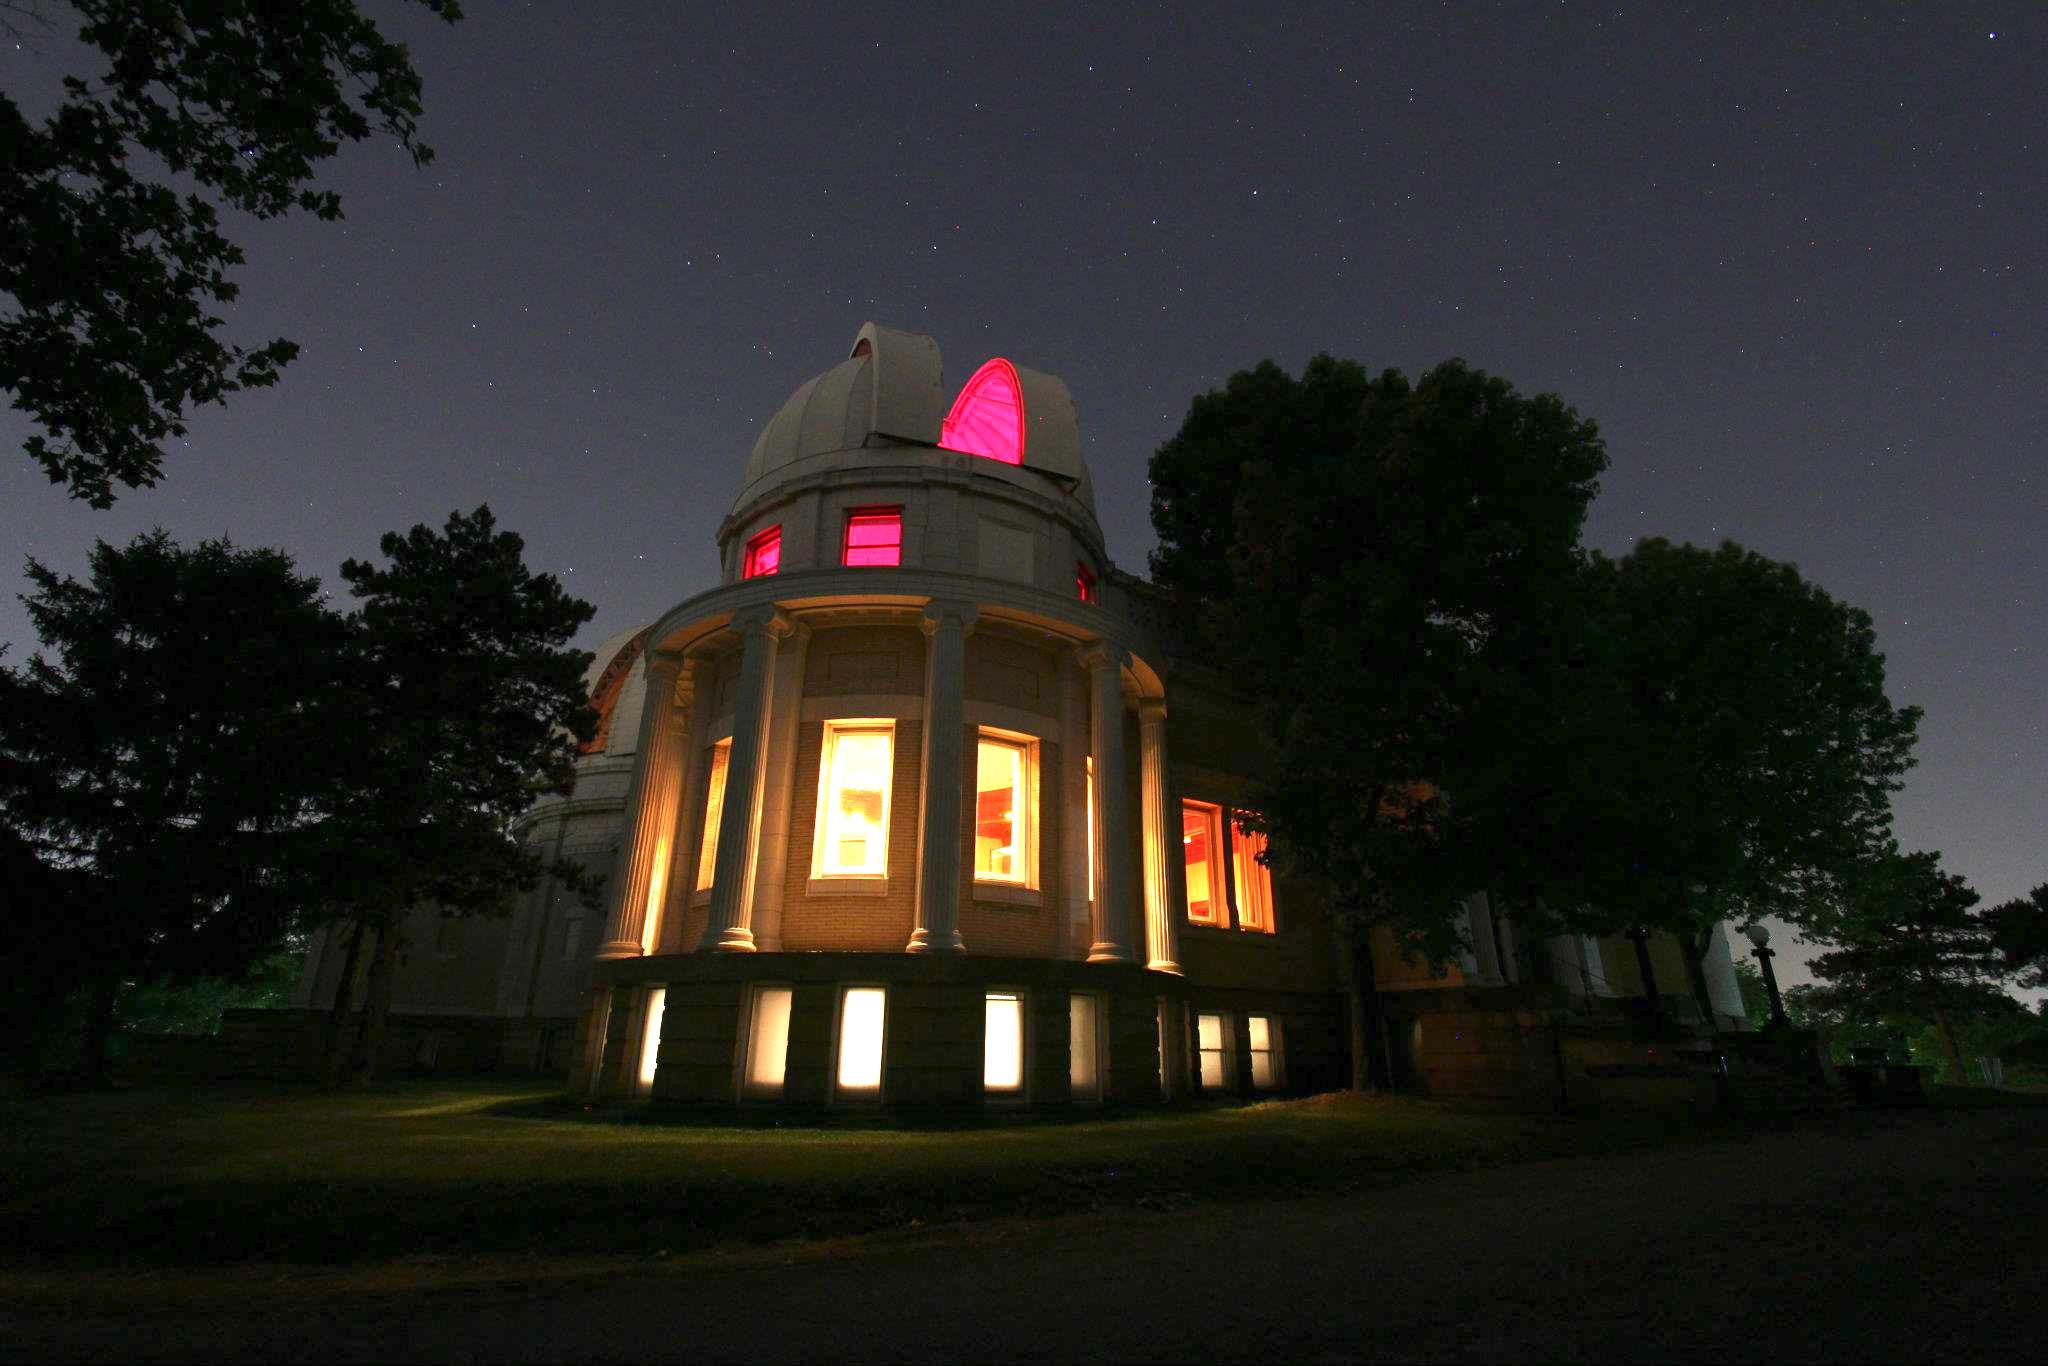
\includegraphics[totalheight=.5\textheight]{Title.jpg}
\end{center}
\begin{center}
\emph{Allegheny Observatory}
\end{center}
\end{figure}

\vfill
\begin{minipage}{0.4\textwidth}
\begin{flushleft}\large
\emph{Authors:}\\
Helena Richie\\
Meghan Cilento
\end{flushleft}
\end{minipage}
\begin{minipage}{0.4\textwidth}
\begin{flushright} \large
\emph{Supervisors:} \\
Professor Wood-Vasey\\
Professor David Turnshek
\end{flushright}
\end{minipage}

\end{center}
\end{titlepage}

%%%%%% Chapter 1: Introduction %%%%%%%%%%%%%%%%%%%%%%%%%%%%%%%%%%
\tableofcontents
\chapter{Introduction}
\parindent0pt

This user's manual provides easy-to-follow instructions on how to run STEPUP Image Analysis (SIA) to generate light curves. SIA was originally written with the intention of generating exoplanet transit light curves for the STEPUP team, however, the program is now generalized to any system which exhibits variations in flux over time. \\

This version of SIA was developed for use in ASTRON 1263. This code has been installed at various locations of use by Pitt's physics students. These locations include the lab room at Allegheny Observatory, the computers in Thaw 210, and the computers in Allen 302. This manual provides separate sections for each of these locations and corresponding instructions on how to run SIA.\\

The main stages of SIA include instrument signature removal from the data (using flat, bias, and dark calibration images), astrometry, and differential aperture photometry. The program requires that these stages run in that order. The calibration and astrometry stages may only be run one time each, however, the final photometry stage may be run multiple times, as long as the first two stages are completed and the data is stored in the proper directories. \\

In addition to the steps needed to run SIA, this manual provides an extensive troubleshooting chapter for each stage as well as a complete flow chart of the entire program. Although this manual should have everything contained within it to successfully run SIA, any questions or comments concerning the user's manual may be directed towards \textbf{Helena Richie (her45@pitt.edu)} or \textbf{Meghan Cilento (mvc27@pitt.edu)}. 


%%%%%% Chapter 2: Preliminary Steps %%%%%%%%%%%%%%%%%%%%%%%%%%%%%%%%%
\chapter{Preliminary Steps}
The preliminary steps to running SIA depend on the location at which it is being run. If you are running SIA from Allegheny Observatory, follow the instructions in Section 2.1. If you are running from Allen 302, follow the instructions in Section 2.2. If you are running from Thaw 210, follow the instructions in Section 2.3. An example of the input file which must be created as a part of the preliminary steps for all locations is shown below. Refer to this image when generating the input file, as proper formatting is required for SIA to run.  \\
%%%%%% General Preliminary Steps %%%%%%%%%%%%%%%%%%%%%%%%%%%%%%%%%%%
\begin{figure}[!h]
\begin{center}
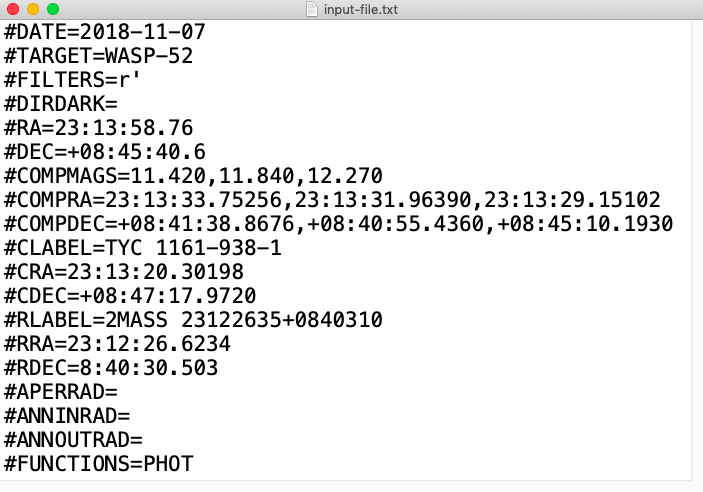
\includegraphics[totalheight=.3\textheight]{example.png}
\caption{Example of input-file.txt}
\label{fig:inputfile}
\end{center}
\end{figure}

\section{Data Configuration}
\label{sect:dataconfig}
\begin{enumerate}
\item All data must be stored in the same directory that is given as input when you run SIA. This includes raw data files, calibration images (including biases, flats, and darks), and the input-file.txt, which the next section explains how to create. {\bf Note:} the dark calibration files \emph{can} be stored in a separate location, but that must be indicated as described in the next section.
\item There are templates for the input file on every computer SIA is installed on. Directions for copying the files are given at the beginning of each location-specific preliminary setup section. It is also quite easy to create one yourself by creating a new text file and filling it in to match Figure \ref{fig:inputfile}.
\item For reference, here is a list of all of the files you need in your raw data directory in order for SIA to run:  \label{itm:filelist}
	\begin{enumerate}
		\item Raw target data.
		\item Three types of calibration files (flats, biases, and darks).
		\item Input file.
		\item \emph{new-image.fits}.
	\end{enumerate}
\end{enumerate}

\section{Creating Input File (General)}
\label{sect:inputfile}
\begin{enumerate}
\item A template for the SIA input file is located in the SIA directory. Copy the input file template to the target directory by typing {\bf copy $\langle$Path to input file$\rangle$ $\langle$Path to target directory$\rangle$}.
\item Make sure you are {\bf cd}'ed into the target's directory by typing \textbf{chdir} and identifying the last directory in the path as the target directory. Once confirmed, type the command {\bf gedit input-file.txt} for Linux or {\bf notepad input-file.txt} for Windows. Now you will begin editing the file.
\item First, enter the absolute file paths for the dark calibration files in the {\bf DIRDARK} keyword. The reason there is a separate keyword for the dark calibration images is because it is common that darks are not taken on the same night as flats and biases. Therefore, these may or may not be stored in the same location as your other calibration files. If they are stored in the same directory as the other calibration files (in the target directory), just leave this entry blank.
\item Go through the file and input all of the parameters that you're immediately aware of. These should include {\bf DATE, TARGET, RA} and {\bf DEC}. the {\bf RA, DEC} keywords correspond to the J2000 RA and Dec of the target.
\item Now that you have completed all of the immediately known entries, you must determine {\bf COMPMAGS, COMPRA, COMPDEC, CLABEL, CRA, CDEC, RLABEL, RRA} and {\bf RDEC}. First, try finding this information in a Variable Star Chart on \emph{aavso.org} by following the next few steps. If you find that a Variable Star Chart does not exist for your target, skip to Step \ref{itm:novsp} and use Aladin Lite to find this information.
\item Once you are on \emph{aavso.org} and logged in, mouse over the \emph{Observing} tab at the top. Under the \emph{Variable Star Charts} option, click on \emph{Variable Star Plotter (VSP)}. 
\item Once on the VSP page, you will need to specify the right ascension and declination of the target, predefined chart scale (which should be option F, 18.5 arcminutes), and the filters which the photometry table should display (at the bottom). Once you have filled out this information, click \emph{Plot Chart} at the bottom.
\item You should have been redirected to a page that has a finder chart for your target on it. At the top under where it says ``Variable Star Plotter" click \emph{Photometry Table for This Chart}.
\item Now, in the {\bf COMPMAGS} category, enter in the magnitudes in the order that they appear, top to bottom, each separated by a comma. \textbf{Important}: be sure to include the magnitude values for only the filter that you observed in. \label{itm:compmags}
\item Also in order from top to bottom, enter the right ascension and declination for each comparison star under the {\bf COMPRA} and {\bf COMPDEC} keywords. They should be in the form {\bf HH:MM:SS} for RA and {\bf DD:MM:SS} for Dec, with each right ascension and declination separated by a comma. There should be no extra spaces before, after, or between any of the entries. \label{itm:compcoord}
\item Now you will need to choose one ``check" star and one ``reference" star that the program will output data on. Choose any two stars in the image of similar magnitudes and location to the target star that have not been used as comparison stars. It does not matter which is which. For each star, enter its name, RA, and Dec into the {\bf CLABEL, CRA, CDEC, RLABEL, RRA}, and {\bf RDEC} categories, respectively. \label{itm:refinf}
\item If AAVSO VSP does not have a Variable Star Chart for your target, then you should use Aladin Lite \emph{https://aladin.u-strasbg.fr/AladinLite/} to find information for your comparison, check, and reference stars. First go to this site and in the box at the top left labeled \emph{Target:}, enter in the target's RA and Dec separated by a comma and a space. Then hit \emph{enter}. \label{itm:novsp}
\item You should now see your target star in the center of the screen. Now, you will have to visually cross-reference stars that you see in the images from the data you are trying to process and the stars in Aladin Lite. Once you have located them in Aladin Lite, select one of the three catalogs seen on the right labeled \emph{SIMBAD}, \emph{GAIA DR2}, and \emph{2MASS}. You should see symbols become overlaid on some or all of the stars in the field of view. You can view information on the star according to that catalog by clicking on the symbol. Your goal is to find information on all of the comparison, check and reference stars from the same catalog and the closest bandpass that you observed in. Choose the catalog that best-fulfills this requirement and record their information as in Steps \ref{itm:compmags}, \ref{itm:compcoord}, and \ref{itm:refinf}.
\item SIA has options to specify aperture and annulus size in the input file. If you would like to enter specific sizes, complete the last three entries {\bf APERRAD, ANNIRAD,} and {\bf ANNOUTRAD}. SIA accepts these keywords in units of arcseconds. If you do not want to specify a specific aperture or annulus size, leave these entries blank. 
\item SIA has two run options: interactive and non-interactive. If you would like to run the program interactively and manually enter commands as the program runs, then it does not matter what you leave in the {\bf FUNCTIONS} entry, as SIA will not use this for anything. If you would like to run the program non-interactively, then in the {\bf FUNCTIONS} keyword enter comma-delimited functions (ISR, ASTROM, and PHOT) in this consecutive order. For example, your line should read {\bf FUNCTIONS=ISR,ASTROM,PHOT} if you would like to run the entire program. 
\item Now that you have completed all of the entries, verify that the file is in your target directory by {\bf cd}ing into your target directory and then using the {\bf dir} command, which will show you everything in the current directory you are in. It should be saved in the directory exactly as \emph{input-file.txt}. If it is named anything other than that, be sure to change it. 
\end{enumerate}

\section{Generating \emph{new-image.fits} File (General)}
\label{sect:newim}
\begin{enumerate}
\item First, open up a browser and go to \emph{astrometry.net}
\item Once on their homepage, select the \emph{use} option. 
\item Now on the \emph{Use the Code} page, select \emph{web}.
\item At the top of the page you're redirected to, select \emph{Upload}. You will go into the directory containing all of your raw data and choose any of the images.
\item Once you have chosen your image, select \emph{Upload}. It will take a minute or so for the image to upload, so don't press anything or leave the page until it does.
\item You will be redirected to a new page. It will usually take only another minute or so for the image to be processed, however it could take longer if the server is busy. Once you see the green \emph{Success} message, click on \emph{Go to results page}.
\item Under the \emph{Calibration} column along the right side, click on \emph{new-image.fits}. This will save the image to the computer's Downloads directory.
\item Move this image into the directory with your instrument signature removed images by typing {\bf mv /home/Downloads/new-image.fits /home/depot/A1263/\emph{data-subdirectory}}.
\end{enumerate}


%%%%%% Preliminary Steps: Allen 302 %%%%%%%%%%%%%%%%%%%%%
\section{Preliminary Steps for Allen 302}

\subsection{Transferring Data}
If your data has been recorded on the Allegheny Observatory Server, but has not yet been transferred to the Astro Computing Server in Allen 302, follow the directions below to do so. The directory in these computers where all ASTRON 1263 data is stored is {\bf /home/depot/A1263}. \newline

\begin{enumerate}
\item Log onto Ptolemy in Allen 302. Open up a terminal window by clicking the terminal icon at the top of the screen. If a directory for your target does not exist, use the {\bf mkdir} command to first make a directory for your target in {\bf /home/depot/A1263} by typing {\bf mkdir /home/depot/A1263/\emph{date-of-observation}}. You may possibly need to specialize a sub-directory further than the date, perhaps by adding one of your group-member's within the date sub-directory if any of your classmates have transferred their own data from this date already.
\item Once there is a directory for your night of observation, use the {\bf cd} command to enter into it. Now, in order to remotely access the data on the observatory computer, type {\bf ftp aoserver1.univ.pitt.edu}. When it prompts you for a name, type \emph{anonymous} and hit enter. When it prompts you for a password, you may type anything and hit enter.
\item Now you must go to the directory from which you wish to transfer data. Do this by typing {\bf cd \emph{date-of-observation}} and whatever sub-directory names that correspond to the location of your data. If you are unsure of this path name, you could check it by following the remote-access instructions in the Observing Guidelines Manual in a separate terminal window and using the file explorer.
\item Before you begin copying files, make sure that prompting is turned off so that you do not have to confirm the transfer of each file individually. Do this by typing {\bf prompt}. The setting toggles between on and off, so you may need to type it twice to make sure it says that prompting is turned off.
\item Next, type {\bf binary}. This changes the mode to transfer.
\item Finally, to copy the files, use the {\bf mget} command. Type {\bf mget \emph{name-of-target}*.fit}. This will transfer all files that have the target name in the title and the ``.fit" extension.
\item Type {\bf bye} to log off of the observatory computer.
\item After typing {\bf bye}, you will automatically revert back to a Ptolemy terminal window. In this window, check to make sure that the files are in the directory that you created by typing {\bf ls}.
\end{enumerate}

\subsection{Creating Input File (Allen 302)}
\begin{enumerate}
\item Now, log off of Ptolemy and log on to Geb, which is located adjacent to Ptolemy on the left.
\item A template of the input file is provided in SIA. Copy the input file template to the target directory by typing {\bf cp /home/depot/STEPUP/input-file.txt /home/depot/A1263/}\newline{\bf \emph{data-subdirectory}}. 
\item Make sure you are {\bf cd}'ed into the target's directory by typing \textbf{pwd}. Once confirmed, type the command {\bf gedit input-file.txt}. Now you will begin editing the file.
\item From here on, you may follow the steps in Section \ref{sect:inputfile}.
\end{enumerate}

\subsection{Generating \emph{new-image.fits} File (Allen 302)}
\label{sect:newim302}
\begin{enumerate}
\item Once you have created the \emph{new-image.fits} file as described in Section \ref{sect:newim}, it will be saved in your Downloads folder. Open up a new terminal window and type the command {\bf mv /home/Downloads/new-image.fits /home/depot/A1263/\emph{data-subdirectory}}.
\end{enumerate}

%%%%%% Preliminary Steps: Allen 302 %%%%%%%%%%%%%%%%%%%%%
\section{Preliminary Steps for Observatory Lab}
\subsection{Creating Input File (Observatory Lab)}
\begin{enumerate}
\item If you are logged onto Ptolemy, you will need to log off and switch to Geb, which is located adjacent to Ptolemy on the left.
\item Open up an Anaconda prompt by going to \emph{Start} $\rightarrow$ \emph{Anaconda Prompt}.
\item A template of the input file is provided in SIA. Copy the input file template to the target directory by typing in the Anaconda Prompt {\bf cp /Z:/SIA\_II/input-file.txt Z:/\emph{data-subdirectory}}.
\item Make sure you are {\bf cd}'ed into the target's directory by typing \textbf{pwd}. Once confirmed, type the command {\bf gedit input-file.txt}. Now you will begin editing the file.
\item From here on, you may follow the steps in Section \ref{sect:inputfile}.
\end{enumerate}

\subsection{Generating \emph{new-image.fits} File (Observatory Lab)}
\begin{enumerate}
\item Once you have created the \emph{new-image.fits} file as described in Section \ref{sect:newim}, it will be saved in your Downloads folder. Open up a new terminal window and type the command {\bf mv Downloads/new-image.fits /Z:/data-subdirectory}.
\end{enumerate}

%%%%%% Chapter 3: Running SIA %%%%%%%%%%%%%%%%%%%%%
\chapter{Running STEPUP Image Analysis}

\section{Program Flow Chart}
\begin{figure}[h!]
\begin{center}
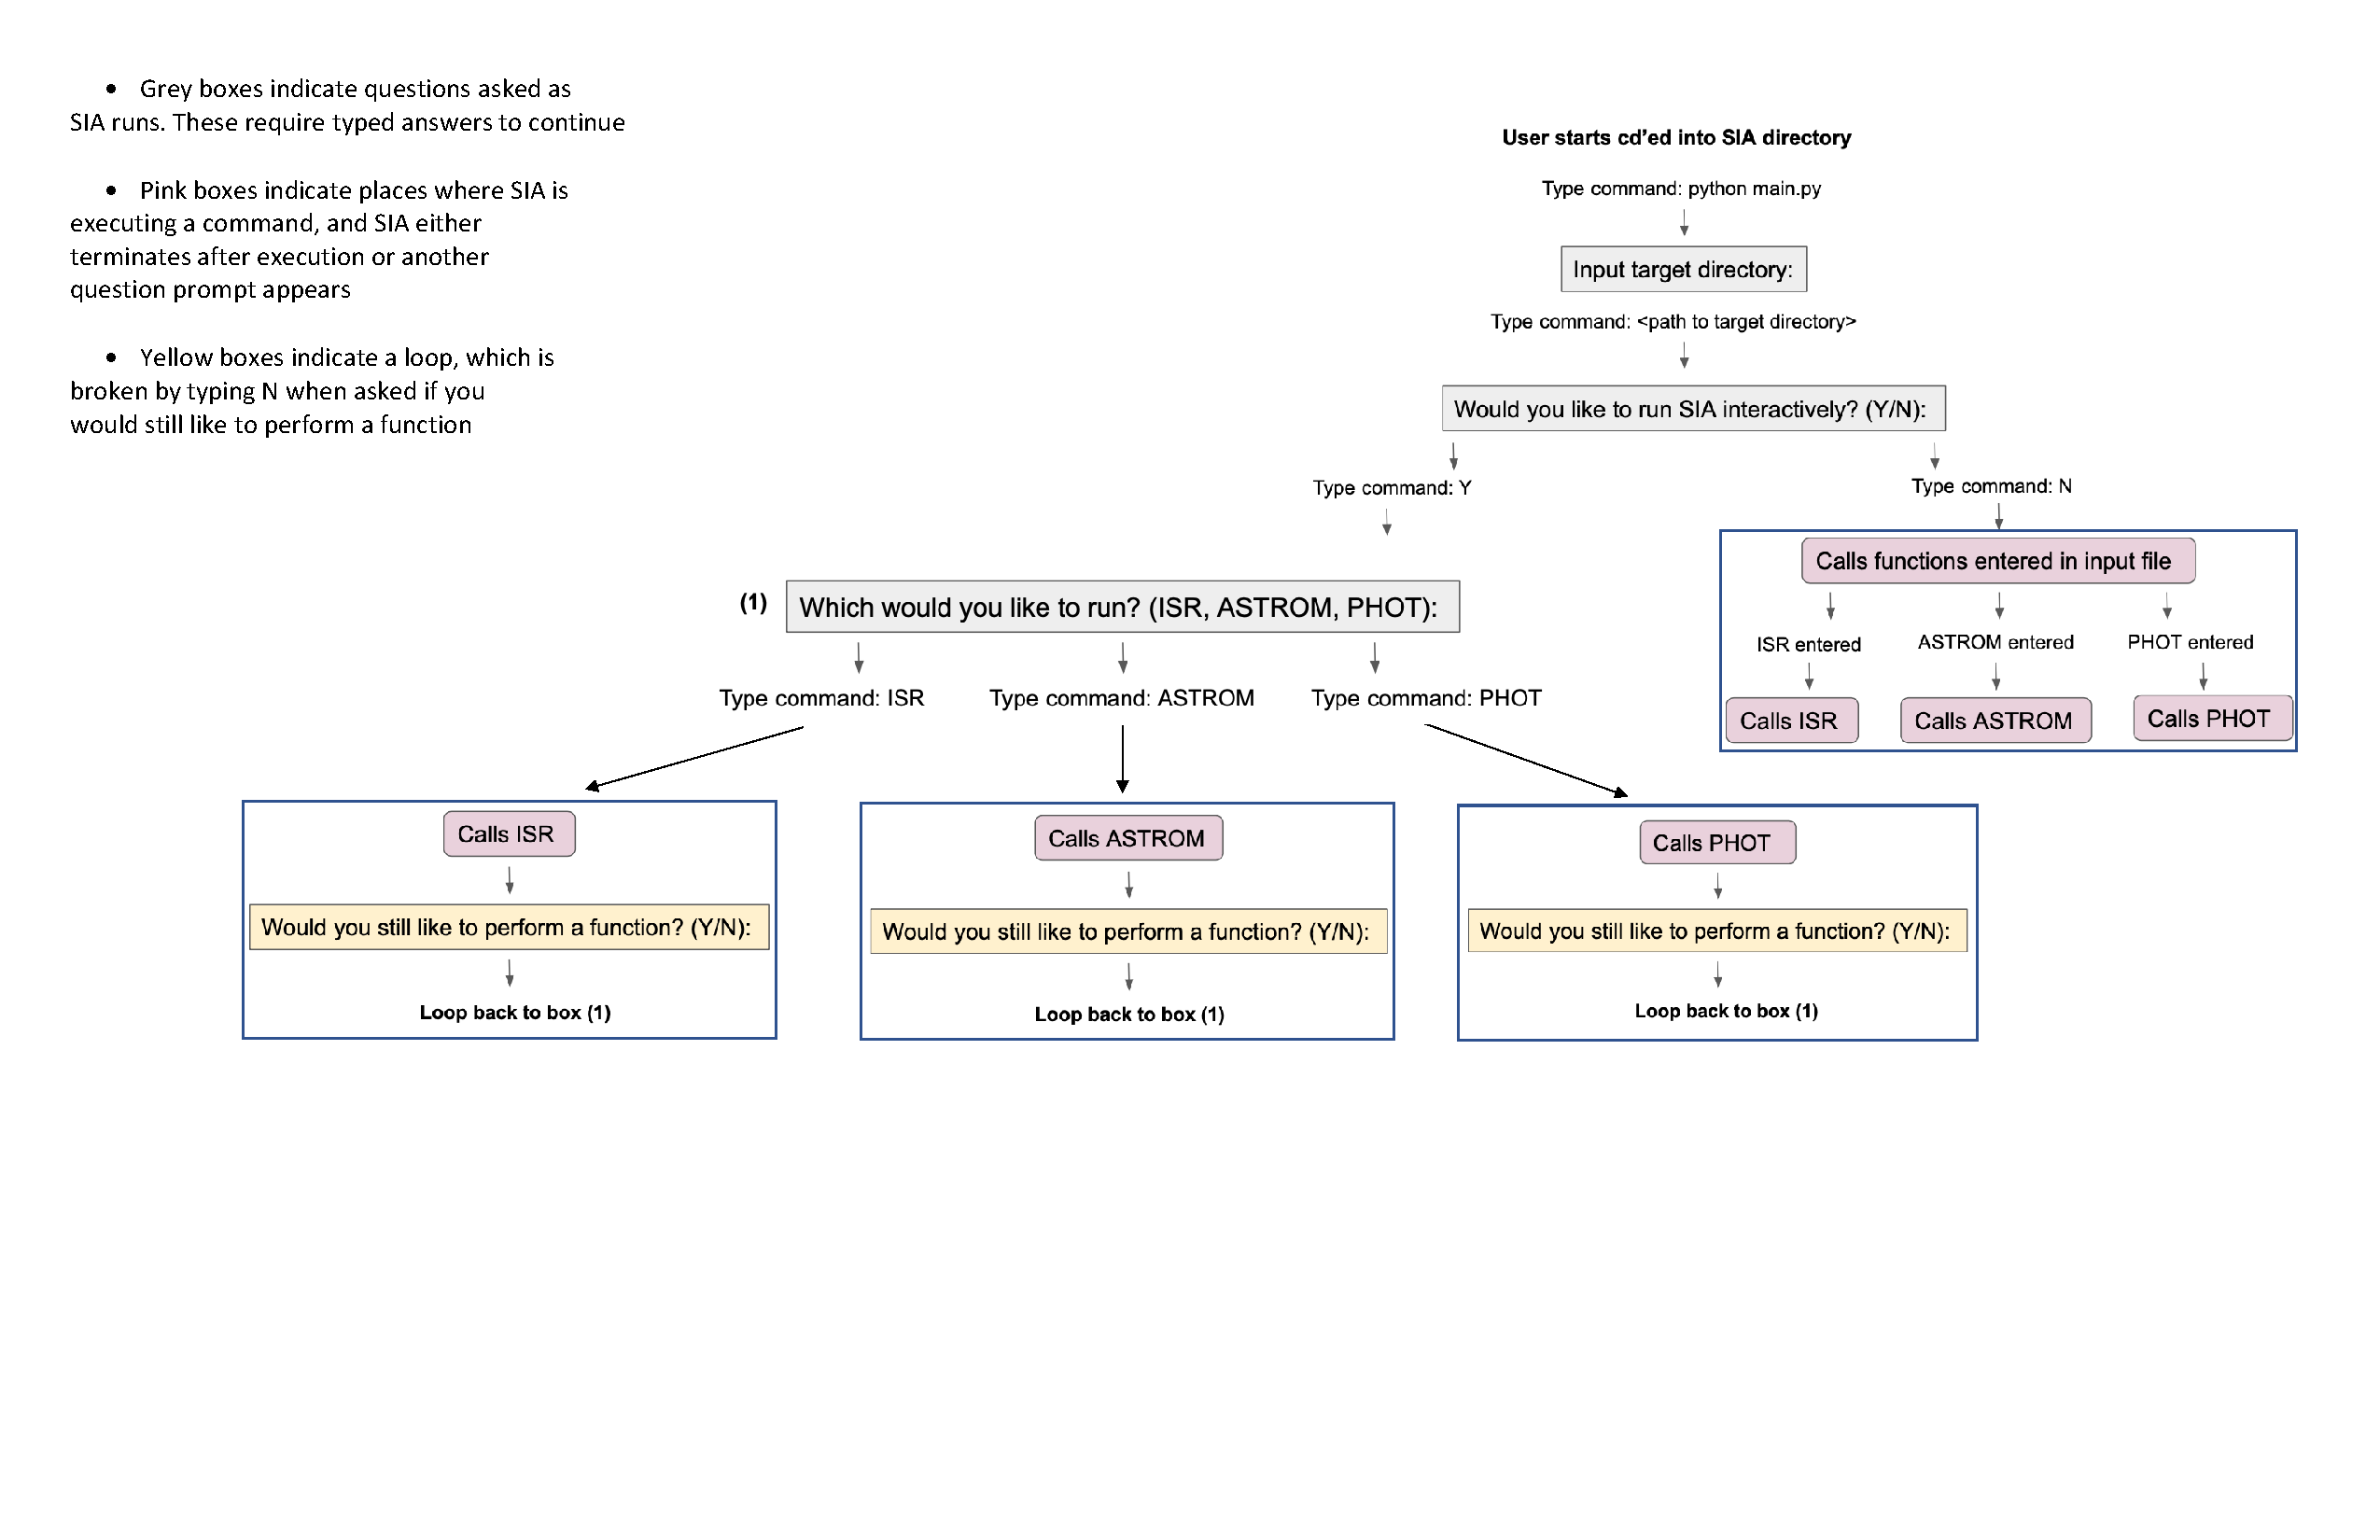
\includegraphics[width=1.3\textwidth,center]{SIA_flow_chart.pdf}
\end{center}
\end{figure}


%%%%%% Running SIA at Allegheny Observatory %%%%%%%%%%%%%%%%
\section{Running at Allegheny Observatory}

\begin{enumerate}
\item This section is specific to running STEPUP Image Analysis in the lab room at Allegheny Observatory. 
\item First, ensure that your data is stored as described in Section \ref{sect:dataconfig}.
\end{enumerate}


%%%%%% Running SIA in Allen 302 %%%%%%%%%%%%%%%%%%%%%
\section{Running in Allen 302}

\begin{enumerate}
\item First, ensure that your data is stored as described in Section \ref{sect:dataconfig}, Item \ref{itm:filelist}.
\item Open up a new terminal window and type {\bf export PATH=\$PATH:/usr/local/wcstools-3.3.3/bin}.
\item The, type the command {\bf scl enable rh-python36 bash} to run Python 3.6.
\item Next, in the same terminal window type {\bf cd /home/depot/STEPUP/STEPUP\_image}\newline{\bf\_analysis\_II}. Now that you have entered into the directory containing the code, type the command {\bf python3 main.py}. This will begin running the code.
\item You will first be asked what directory your data is contained in. This should be a sub-directory in {\bf /home/depot/A1263}. Enter the absolute path to that directory (case-sensitive).
\item Next, you will be asked whether you would like to run SIA interactively or not. If so, enter {\bf Y}. If not, enter {\bf N} and SIA will begin to run whatever functions you specified in the \emph{input-file.txt} (case-sensitive).
\item If you are running SIA interactively, you will next be asked which of the three functions you would like to run, \emph{ISR, ASTROM,} or \emph{PHOT}. Keep in mind that if you have not processed any data yet, you will need to run each function successively. Once you have ran \emph{ISR} and \emph{ASTROM} once you may not run them again (unless you remove all of the output they generated) and you may run \emph{PHOT} as many times as you wish. Enter the function you wish to run as {\bf ISR}, {\bf ASTROM}, or {\bf PHOT}. \label{itm:whichfunc}
\item Now, SIA should be running whichever function you entered.
\item Once the function is finished running, you will be asked if you would like to perform another function. If so, enter {\bf Y}. Then you will be asked which function you would like to run as in Step \ref{itm:whichfunc}. Enter your response according to the description in this step. If you are finished running SIA, enter {\bf N} and SIA will print \emph{Goodbye.} and you will be returned to the terminal command prompt.
\end{enumerate}

\subsection{Generating a Color Light Curve}
\begin{enumerate}
\item If you observed in two different filters, then you have the option to generate a color light curve. In this case, when running \emph{PHOT}, SIA will ask you if you would like to generate a color light curve. If so, enter {\bf Y}. Then you will be asked which filters you would like to generate the light curve for. Enter the filters as they are given in the headers of the FITS files in the order you would like to subtract them separated by a comma with no spaces. For example, entering {\bf g',r'} corresponds to generating a light curve of $\textrm{g'}-\textrm{r'}$ color.
\end{enumerate}

%%%%%% Running SIA in Thaw 210 %%%%%%%%%%%%%%%%%%%%%
%\section{Running in Thaw 210}

%\begin{enumerate}
%\item This section is specific to running STEPUP Image Analysis on the computers provided in Thaw 210. 
%\end{enumerate}

%%%%%% Chapter 5: Troubleshooting %%%%%%%%%%%%%%%%%%%%%
\chapter{Troubleshooting}

\emph{Note:} STEPUP Image Analysis was written in 2017 in Python 3.6.2. The Troubleshooting tips below are written in accordance with the Python 3.6.2 documentation and syntax. 

\section{Instrument Signature Removal}
\begin{enumerate}
\item {\bf NotADirectoryError}: If you get an error telling you that a certain directory does not exist, it is most likely because you typed something wrong (i.e. capitalizing/not capitalizing letters that should be capital or adding additional spaces). Simply type {\bf python3 main.py} to try again and by \emph{very careful} to make sure you are typing the data directory as you would to {\bf cd} to it in a terminal window, since that is essentially what SIA is doing.
\item {\bf IsADirectoryError}
\item {\bf KeywordError}
\end{enumerate}
\section{Perform Astrometry}
\begin{enumerate}
\item {\bf IsADirectoryError}
\end{enumerate}
\section{Perform Photometry}
\begin{enumerate}
\item Outlier points.
\item Different number of images in one filter than the other.
\item Including test images in sequence (different exposure times).
\item Comparison/check/reference stars not in the image.
\item Saturated images.
\end{enumerate}

%%%%%%%%%%%%%%%%%%%%%%%%%%%%%%%%%%%%%%%%%%%%%%%%%%%%%%%%%%%%%%
\end{document}